\documentclass[handout]{beamer}
%\documentclass{article}
\usepackage{animate}
\usepackage{xcolor}
\usepackage{amsmath}
\usepackage{array}
\usepackage{graphicx}
\setbeamertemplate{navigation symbols}{}
\setbeamertemplate{caption}{\insertcaption} \setbeamertemplate{caption label separator}{}
\renewcommand{\emph}{\textbf}
\usetheme{Warsaw}
\title{Ch. 5 -- Joint Probability Distributions}
%\setlength{\parskip}{.2cm}
\DeclareMathOperator{\Bin}{Bin}
\DeclareMathOperator{\Cov}{Cov}
\DeclareMathOperator{\Corr}{Corr}
\DeclareMathOperator{\Var}{Var}
\begin{document}
\begin{frame}
\begin{beamercolorbox}[rounded=true,wd=\textwidth,center]{title}
\usebeamerfont{title}\inserttitle
\end{beamercolorbox}
\begin{center}
% \includegraphics[scale=.7]{comics/correlation.png}
\end{center}
\end{frame} 

\begin{frame}{Joint Probability Mass Function}
\begin{block}{}
Let $X$ and $Y$ be discrete random variables. Their \emph{joint probability mass function} (joint pmf) is
$$f(x,y) = P(X=x \cap Y=y)$$

\end{block}

\pause Example: A insurance agency serves many customers with both an automobile policy and a homeowner’s policy. The possible amounts for a deductible are \$100 and \$250 for an automobile policy, and \$0, \$100, and \$200 for a homeowner's policy. If a customer is selected at random, and $X$ is their deductible on the auto policy and $Y$ is their deductible on the homeowner’s policy, then the joint pmf of $X$ and $Y$ may be described by a table such as the following:
\begin{center}
\begin{tabular}{l||l|l|l}
$f(x,y)$ & $y=0$ & $y=100$ & $y=200$ \\ \hline \hline
$x=100$ & .20 & .10 & .20 \\ \hline
$x=250$ & .05 & .15 & .30
\end{tabular}
\end{center}
\end{frame}

\begin{frame}{Example}
\begin{block}{}
Suppose we roll two fair 6-sided dice, and let $X$ be the smaller of the two rolls, and let $Y$ be the larger. Find the joint probability mass function $f(x,y)$ of $X$ and $Y$.
\end{block}
\pause
\begin{center}
\begin{tabular}{l||l|l|l|l|l|l}
$f(x,y)$ & $y=1$ & $y=2$ & $y=3$ & $y=4$ & $y=5$ & $y=6$ \\ \hline\hline
$x=1$ & 1/36 & 2/36 & 2/36 & 2/36 & 2/36 & 2/36 \\ \hline
$x=2$ & 0 & 1/36 & 2/36 & 2/36 & 2/36 & 2/36 \\ \hline
$x=3$ & 0 & 0 & 1/36 & 2/36 & 2/36 & 2/36 \\ \hline
$x=4$ & 0 & 0 & 0 & 1/36 & 2/36 & 2/36 \\ \hline
$x=5$ & 0 & 0 & 0 & 0 & 1/36 & 2/36 \\ \hline
$x=6$ & 0 & 0 & 0 & 0 & 0 & 1/36
\end{tabular}
\end{center}

For instance, $f(2,3)=2/36$, but $f(3,2)=0$.
\end{frame}

\begin{frame}{Marginal Probability Mass Function}
\begin{block}{}
Let $X$ and $Y$ be discrete random variables with joint probability mass function $f(x,y)$. The \emph{marginal probability mass function} of $X$ is defined as
$$f_X(x) = \sum_y f(x,y)$$
where the sum is taken over all possible values of $Y$. Similarly, the marginal probability mass function of $Y$ is
$$f_Y(y) = \sum_x f(x,y)$$
where the sum is taken over all possible values of $X$.
\end{block}

Note: $f_X$ is simply the probability mass function of $X$ considered as a random variable on its own: $f_X(x) = P(X=x)$.
\end{frame}

\begin{frame}{Example}
Recall the joint pmf for the auto insurance deductible $X$ and homeowner's insurance deductible $Y$ from earlier:
\begin{center}
\begin{tabular}{l||l|l|l}
$f(x,y)$ & $y=0$ & $y=100$ & $y=200$ \\ \hline \hline
$x=100$ & .20 & .10 & .20 \\ \hline
$x=250$ & .05 & .15 & .30
\end{tabular}
\end{center}
\pause The marginal pmf for the auto insurance deductible $X$ is given by
\begin{align*}
f_X(100) &= .50 \\
f_X(250) &= .50
\end{align*}
\pause The marginal pmf for the homeowner's deductible $Y$ is given by
\begin{align*}
f_Y(0) &= .25 \\
f_Y(100) &= .25 \\
f_Y(200) &= .50
\end{align*}
\end{frame}

\begin{frame}{Independence of Random Variables}
\begin{block}{}
Discrete random variables $X$ and $Y$ are \emph{independent} if their joint probability mass function $f(x,y)$ is the product of the marginal probability mass functions $f_X(x)$ and $f_Y(y)$:
$$f(x,y) = f_X(x)f_Y(y)$$
\end{block}

In the insurance example,
\begin{center}
\begin{tabular}{l||l|l|l}
$f(x,y)$ & $y=0$ & $y=100$ & $y=200$ \\ \hline \hline
$x=100$ & .20 & .10 & .20 \\ \hline
$x=250$ & .05 & .15 & .30
\end{tabular}
\end{center}
the random variables $X$ and $Y$ are dependent, because, e.g.,
$$f(100,0) = .20 \neq (.50)(.25) = f_X(100)f_Y(0)$$
\end{frame}

\begin{frame}{Example}
\begin{block}{}
If $X$ and $Y$ are independent geometric random variables with parameter $p$ and $q$ respectively, find the joint pmf of $X$ and $Y$.
\end{block}
\pause Solution: The marginal pmf of $X$ is
$$f_X(x) = p(1-p)^x$$
\pause while the marginal pmf of $Y$ is
$$f_Y(y) = q(1-q)^y$$
\pause Since $X$ and $Y$ are independent, their joint pmf is the product of their marginal pmfs:
$$f(x,y) = f_X(x)f_Y(y) = p(1-p)^xq(1-q)^y$$
\end{frame}

%\begin{frame}{Conditional Probability Mass Function}
%\begin{block}{}
%Let $X$ and $Y$ be random variables with joint pmf $f(x,y)$. The \emph{conditional probability mass function} of $Y$ given $X$ is
%$$f_{Y\mid X}(y\mid x) = \frac{f(x,y)}{f_X(x)}$$
%\end{block}
%\pause The conditional pmf may be expressed in terms of conditional probabilities:
%$$f_{Y\mid X}(y\mid x) = P(Y=y \mid X=x)$$
%\pause If $X$ and $Y$ are independent, then the conditional pmf of $Y$ given $X$ is simply the marginal pmf of $Y$:
%$$f_{Y\mid X}(y\mid x) = \frac{f(x,y)}{f_X(x)} = \frac{f_X(x)f_Y(y)}{f_X(x)} = f_Y(y)$$
%\end{frame}

%\begin{frame}{Example}
%In the insurance example, the auto deductible $X$ and homeowner's deductible $Y$ had joint pmf given by
%
%\begin{center}
%\begin{tabular}{l||l|l|l}
%$f(x,y)$ & $y=0$ & $y=100$ & $y=200$ \\ \hline \hline
%$x=100$ & .20 & .10 & .20 \\ \hline
%$x=250$ & .05 & .15 & .30
%\end{tabular}
%\end{center}
%
%Find the conditional pmf of homeowner's deductible $Y$, given the auto deductible $X$ is \$100:
%
%\vspace{.2cm}
%\pause
%Solution: 
%\begin{align*}
%f_{Y\mid X}(0 \mid 100) &= \frac{f(100,0)}{f_X(100)} = \frac{.20}{.50} = .40\\
%f_{Y\mid X}(100 \mid 100) &= \frac{f(100,100)}{f_X(100)} = \frac{.10}{.50} = .20\\
%f_{Y\mid X}(200 \mid 100) &= \frac{f(100,200)}{f_X(100)} = \frac{.20}{.50} = .40
%\end{align*}
%\end{frame}

\begin{frame}{Sum of Two Discrete Random Variables}
\begin{block}{}
Given random variables $X$ and $Y$ with joint pmf $f(x,y)$, the sum $X+Y$ has pmf
$$f_{X+Y}(t) = \sum f(x,t-x)$$
where the sum is taken over all possible values $x$ of $X$. 
\end{block}

\vspace{.2cm}\pause
In particular, if $X$ and $Y$ are independent, then
$$f_{X+Y}(t) =\sum f_X(x)f_Y(t-x)$$
\end{frame}

\begin{frame}{Example}
\begin{block}{}
Suppose $X$ and $Y$ are independent geometric random variables with parameters $p=.3$ and $q=.4$ respectively. What is the probability that $X+Y=2$?
\end{block}
\pause Solution: The marginal pmfs are $f_X(x)=p(1-p)^x$ and $f_Y(y)=q(1-q)^y$. \pause Therefore,
\begin{align*}
&P(X+Y=2) \\
&= \sum_x f_X(x)f_Y(2-x) \\
\uncover<4->{&= f_X(0)f_Y(2) + f_X(1)f_Y(1) + f_X(2)f_Y(0) \\}
\uncover<5->{&= p(1-p)^0q(1-q)^2 + p(1-p)^1q(1-q)^1+p(1-p)^2q(1-q)^0 \\}
\uncover<6->{&= (.3)(.4)(.6)^2 + (.3)(.7)(.4)(.6) + (.3)(.7)^2(.4) }
\uncover<7->{= .1524}
\end{align*}
\end{frame}

\begin{frame}{Expected Value}
\begin{block}{}
Given random variables $X$ and $Y$ with joint pmf $f(x,y)$, and given a function $h(x,y)$, the \emph{expected value} of $h(X,Y)$ is
$$E[h(X,Y)] = \sum_x\sum_y h(x,y)f(x,y)$$
where the sums are over the possible values for $X$ and $Y$.
\end{block}
\pause Example: If $X$ and $Y$ are the auto and homeowner's insurance deductible as before, find the expected value of $|X-Y|$:
\pause \begin{align*}
E(|X-Y|) &= \sum_x\sum_y |x-y|f(x,y) \\
\uncover<4->{&= |100-0|(.20) + |100-100|(.10) + |100-200|(.20) \\
&\  + |250-0|(.05) + |250-100|(.15)+|250-200|(.30) \\}
\uncover<5->{&= 90}
\end{align*}
\end{frame}

\begin{frame}{Several Random Variables}
If $X_1, \dots, X_n$ are random variables, their joint pmf is defined as
$$f(x_1,\dots,x_n) =P(X_1=x_1, \dots, X_n=x_n)$$
\pause The marginal pmf of $X_1$ is defined as
$$f_{X_1}(x)= \sum_{x_2}\sum_{x_3}\cdots\sum_{x_n} P(X_1=x, X_2=x_2,\dots,X_n=x_n)$$
\pause The random variables $X_1,\dots,X_n$ are independent if
$$f(x_1,x_2,\dots,x_n) = f_{X_1}(x_1)f_{X_2}(x_2)\cdots f_{X_n}(x_n)$$
\end{frame}

\begin{frame}{Problem}
\begin{block}{}
A manufacturer receives components of a certain type from 3 plants: 50\% from plant A, 30\% from plant B, 20\% from plant C. If you randomly select 9 of these components, what is the probability that exactly three would come from each plant?
\end{block}

\pause Solution: There are many ways that 3 components could come from each plant, e.g., the sources of the 9 components could be ABBACCBAC. The possible ways correspond to  rearrangements of the ``word" AAABBBCCC, of which there are $\frac{9!}{3!3!3!}=1680$.

\vspace{.2cm}
\pause Therefore the probability that exactly 3 components would come from each plant is
$$1680P(AAABBBCCC) = 1680(.5)^3(.3)^3(.2)^3 =  .04536$$
\end{frame}

\begin{frame}{Multinomial Distribution}
The previous problem can be generalized:
\begin{block}{}
Suppose a sequence of independent random variables $Y_1,\dots,Y_n$ each have $r$ possible values with probabilities $p_1,\dots,p_r$. Let $X_i$ be the number of $Y_1,\dots,Y_n$ which have value $i$. Then $(X_1,\dots,X_r)$ have a \emph{multinomial} distribution. The joint pmf is
$$f(x_1,\dots,x_r) = \begin{cases}\frac{n!}{x_1!\cdots x_r!}p_1^{x_1}\cdots p_r^{x_r}, & \text{if }x_1+\cdots+x_r=n \\ 0, & \text{otherwise}\end{cases}$$
\end{block}
\pause When there are only two possible outcomes ($r=2$), this reduces to a binomial distribution:
$$f(x,n-x) = \frac{n!}{x!(n-x)!}p_1^xp_2^{n-x} = \binom n x p_1^x(1-p_1)^{n-x}$$
\end{frame}

\begin{frame}{Joint Probability Density}
\begin{block}{}
Random variables $X$ and $Y$ are said to have a \emph{joint probability density} (joint pdf) $f(x,y)$ if
$$P(a \leq X \leq b, c \leq Y \leq d) = \int_a^b\int_c^d f(x,y)\ dy\ dx$$
for all real constants $a\leq b$ and $c\leq d$.
\end{block}
To be a valid joint pdf, we must have $\int_{-\infty}^\infty\int_{-\infty}^\infty f(x,y)\ dy\ dx=1$.
\end{frame}

\begin{frame}{Example}
\begin{block}{}
A bank operates a drive-up facility and a walk-up window. On a random day, let $X$ be the proportion of time the drive-up facility is in use, and let $Y$ be the proportion of time the walk-up window is in use. Check that a valid joint pdf for $X$ and $Y$ is given by
$$f(x,y)=\begin{cases}\frac65(x+y^2), & 0\leq x \leq 1, 0\leq y\leq 1 \\ 0, & \text{otherwise}\end{cases}$$
\end{block}
\vspace{-.2cm}\pause \begin{align*}
\int_{-\infty}^\infty\int_{-\infty}^\infty f(x,y)\ dy\ dx &= \int_0^1\int_0^1 \frac65(x+y^2)\ dy\ dx \\
\uncover<3->{&=\frac65 \int_0^1 \left(xy+\frac{y^3}3\right)\Big\vert_{y=0}^1\ dx \\}
\uncover<4->{&= \frac65\int_0^1 \left(x+ \frac13\right)\ dx}
\uncover<5->{= \frac65\left(\frac12+\frac13\right) }
\uncover<6->{= 1}
\end{align*}
\end{frame}

\begin{frame}{Marginal Probability Density Function}
\begin{block}{}
Let $X$ and $Y$ be random variables with joint pdf $f(x,y)$. The \emph{marginal probability density function} (marginal pdf) of $X$ is defined as
$$f_X(x) = \int_{-\infty}^\infty f(x,y)\ dy$$
Similarly, the marginal pdf of $Y$ is
$$f_Y(y) = \int_{-\infty}^\infty f(x,y)\ dx$$
\end{block}

\pause Note: $f_X$ is simply the pdf of $X$ considered as a random variable on its own.

\pause\begin{block}{}
 $X$ and $Y$ are independent if their joint pdf is the product of the marginal pdfs:
$$f(x,y) = f_X(x)f_Y(y)$$
\end{block}
\end{frame}

\begin{frame}{Example}
\begin{block}{}
In the bank example, the joint pdf of two random variables $X$ and $Y$ was given by
$$f(x,y)=\begin{cases}\frac65(x+y^2), & 0\leq x \leq 1, 0\leq y\leq 1 \\ 0, & \text{otherwise}\end{cases}$$
Find the marginal pdf of $X$.
\end{block}
\pause \vspace{-.2cm}\begin{align*}
f_X(x) &= \int_{-\infty}^\infty f(x,y)\ dy \\
\uncover<3->{&= \int_0^1 \frac65(x+y^2)\ dy \\}
\uncover<4->{&= \frac65\left(xy+\frac{y^3}3\right)\Big\vert_{y=0}^1}
\uncover<5->{= \frac65\left(x+\frac13\right)}
\end{align*}
\end{frame}

\begin{frame}{Example}
\begin{block}{}
A system has two components; assuming their lifetimes $X$ and $Y$ are independent exponential random variables with $E(X)=10$ and $E(Y)=20$, what is the probability that the first component outlasts the second?
\end{block}

\pause\vspace{-.2cm}
\begin{tabular}{p{7.2cm}p{4cm}}
\vspace{0cm}$\begin{aligned}[t]
P(X\geq Y) &= \int_0^\infty\int_y^\infty f(x,y)\ dx\ dy \\
\uncover<3->{&= \int_0^\infty\int_y^\infty \frac1{200}e^{-\frac{x}{10}-\frac{y}{20}}\ dx\ dy \\}
\uncover<4->{&= \frac1{200}\int_0^\infty e^{-y/20}\int_y^\infty e^{-x/10}\ dx\ dy \\}
\uncover<5->{&= \frac1{200}\int_0^\infty e^{-y/20}\cdot 10e^{-y/10}\ dy \\}
\uncover<6->{&= \frac1{20}\int_0^\infty e^{-\frac3{20}y}\ dy }
\uncover<7->{= \frac1{20}\cdot \frac{20}3 }
\uncover<8->{= \frac13}
\end{aligned}$
& \vspace{-.2cm}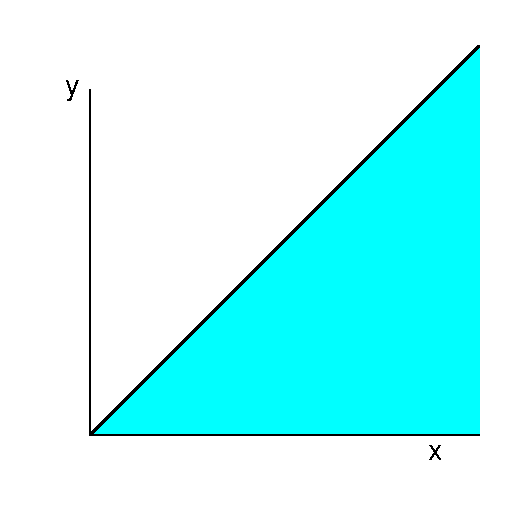
\includegraphics[scale=.4]{ch5_xy.pdf}
\end{tabular}
\end{frame}

%\begin{frame}{Conditional Probability Density Function}
%\begin{block}{}
%Let $X$ and $Y$ be random variables with joint pdf $f(x,y)$. The \emph{conditional probability density function} of $Y$ given $X$ is
%$$f_{Y\mid X}(y\mid x) = \frac{f(x,y)}{f_X(x)}$$
%\end{block}
%\pause If $X$ and $Y$ are independent, then the conditional pdf of $Y$ given $X$ is simply the marginal pdf of $Y$:
%$$f_{Y\mid X}(y\mid x) = \frac{f(x,y)}{f_X(x)} = \frac{f_X(x)f_Y(y)}{f_X(x)} = f_Y(y)$$
%\end{frame}

\begin{frame}{Sum of Two Continuous Random Variables}
Recall that for discrete random variables $X$ and $Y$ with joint pmf $f(x,y)$, their sum $X+Y$ has pmf
$$f_{X+Y}(t) = \sum_x f(x,t-x)$$
\pause\vspace{-.3cm} \begin{block}{}
Given continuous random variables $X$ and $Y$ with joint pdf $f(x,y)$, their sum $X+Y$ has pdf
$$f_{X+Y}(t) = \int_{-\infty}^\infty f(x,t-x)\ dx$$
\end{block}
In particular, if $X$ and $Y$ are independent, then
$$f_{X+Y}(t) = \int_{-\infty}^\infty f_X(x)f_Y(t-x)\ dx$$
\end{frame}

\begin{frame}{Sum of Independent Normal Random Variables}
With a bit of calculus and algebra, one may show:
\begin{block}{}
If $X$ and $Y$ are independent normal random variables, 
%$X\sim N(\mu_1,\sigma_1^2)$, $Y\sim N(\mu_2,\sigma_2^2)$, 
then their sum $X+Y$ is also a normal random variable.
% \begin{align*}
%X+Y&\sim N(\mu_1+\mu_2,\sigma_1^2+\sigma_2^2)
%X-Y &\sim N(\mu_1-\mu_2,\sigma_1^2+\sigma_2^2)
%\end{align*}
\end{block}
\pause If $X\sim N(\mu_1,\sigma_1^2)$ and $Y\sim N(\mu_2,\sigma_2^2)$, then
\begin{align*}
E(X+Y)&=E(X)+E(Y)=\mu_1+\mu_2 \\
V(X+Y)&=V(X)+V(Y)=\sigma_1^2+\sigma_2^2
\end{align*}
So $X+Y\sim N(\mu_1+\mu_2,\sigma_1^2+\sigma_2^2)$.

\vspace{.2cm}
\pause Note: Since $Y$ is normal, $-Y$ is normal, $-Y\sim N(-\mu_2,\sigma_2^2)$, so the difference $X-Y$ is also normal: $X-Y\sim N(\mu_1-\mu_2,\sigma_1^2+\sigma_2^2)$.

%\begin{align*}
%f_{X+Y}(t) &= (f_X * f_Y)(t) \\
%&= \int_{-\infty}^\infty f_X(x)f_Y(t-x)\ dx \\
%&= \int_{-\infty}^\infty \frac1{\sigma_1\sqrt{2\pi}}e^{-x^2/2\sigma_1^2} \frac1{\sigma_2\sqrt{2\pi}}e^{-(t-x)^2/2\sigma_2^2}\ dx \\
%&= \frac1{\sigma_1\sigma_2\cdot2\pi} e^{-t^2/2\sigma_2^2} \int_{-\infty}^\infty e^{-\frac{\sigma_2^2x^2+\sigma_1^2x^2-2t\sigma_1x}{2\sigma_1^2\sigma_2^2}}\ dx \\
%\end{align*}
\end{frame}


\begin{frame}{Example}
\begin{block}{}
Suppose that the height of a randomly selected male adult in the US is normal with mean $\mu=69.5$ inches and standard deviation $\sigma=1.9$ inches. If two individuals from this population are selected at random, what is the probability that their height differs by more than 4 inches?
\end{block}
\pause Solution: If the two individuals have heights $X$ and $Y$, then $X, Y\sim N(69.5,1.9^2)$, and so $$X-Y \sim N(69.5-69.5, 1.9^2+1.9^2) = N(0,7.22)$$
\pause Thus $X-Y$ is normal with mean 0 and standard deviation $\sigma=\sqrt{7.22}\approx 2.687$.
\pause \begin{align*}
P(|X-Y| > 4) &\approx P(|Z| > 4/2.687) \\
&\approx P(|Z| > 1.49) \\
&= 2P(Z<-1.49) = 2(.0681) = .1362
\end{align*}
\end{frame}

\begin{frame}{Covariance}
\begin{block}{}
Given random variables $X$ and $Y$ with means $\mu_X$ and $\mu_Y$ respectively, their \emph{covariance} is
$$\Cov(X,Y) = E[(X-\mu_X)(Y-\mu_Y)]$$
\end{block}
\pause As for variance, there is a shortcut formula for covariance:
$$\Cov(X,Y) = E(XY) - E(X)E(Y)$$
\pause The covariance has several useful properties: 
\begin{block}{}
\begin{enumerate}
\item $\Cov(X,X) = V(X)$
\item $\Cov(Y,X) = \Cov(X,Y)$
\item $\Cov(cX,Y) = c\Cov(X,Y)$
\item $\Cov(X+Y,Z) = \Cov(X,Z)+\Cov(Y,Z)$
\end{enumerate}
\end{block}
%\pause Proof: 
%\begin{align*}
%\Cov(X,Y) &= E[(X-\mu_X)(Y-\mu_Y)] \\
%\uncover<4->{&= E[XY - \mu_XY-\mu_YX+\mu_X\mu_Y] \\}
%\uncover<5->{&= E(XY) - \mu_XE(Y) - \mu_YE(X) + \mu_X\mu_Y \\}
%\uncover<6->{&= E(XY) - E(X)E(Y) - E(Y)E(X) + E(X)E(Y) \\}
%\uncover<7->{&= E(XY) - E(X)E(Y)}
%\end{align*}
\end{frame}

\begin{frame}{Correlation}
\begin{block}{}
The \emph{correlation} between two random variables $X$ and $Y$ is 
$$\rho = \Corr(X,Y) = \frac{\Cov(X,Y)}{\sqrt{V(X)}\sqrt{V(Y)}} = \frac{\Cov(X,Y)}{\sigma_X\sigma_Y}$$
\end{block}
Correlation is a measure of how strongly related two random variables are. \pause It has several properties:
\begin{block}{}
\begin{enumerate}
\item $-1 \leq \rho \leq 1$
\item  If $X$ and $Y$ are independent, then $\Corr(X,Y)=0$.
\item Changing the scale of $X$ and/or $Y$ does not affect the correlation, i.e. for any $c\neq 0$,
$$\Corr(cX,Y) = \Corr(X,Y) = \Corr(X,cY)$$
\end{enumerate}
\end{block}
\end{frame}

\begin{frame}{Example}
\begin{block}{}
In the bank example, the joint pdf of two random variables $X$ and $Y$ was given by
$$f(x,y)=\begin{cases}\frac65(x+y^2), & 0\leq x \leq 1, 0\leq y\leq 1 \\ 0, & \text{otherwise}\end{cases}$$
Find the correlation of $X$ and $Y$.
\end{block}
\pause The marginal pdfs of $X$ and $Y$ are, for $0\leq x \leq 1, 0\leq y\leq 1$,
\begin{align*}
f_X(x) &= \int_0^1 \frac65(x+y^2)\ dy
= \frac65\left(xy+\frac{y^3}3\right)\Big\vert_{y=0}^1
= \frac65\left(x+\frac13\right) \\
f_Y(y) &= \int_0^1\frac65(x+y^2)\ dx = \frac65\left(\frac{x^2}2+xy^2\right)\Big\vert_{x=0}^1=\frac65\left(\frac12+y^2\right)
\end{align*}
\end{frame}

\begin{frame}{Example (continued)}
From the marginal pdfs $f_X(x)=\frac65(x+\frac13)$ and $f_Y(y)=\frac65(\frac12+y^2)$,
\begin{align*}
E(X) &= \int_{-\infty}^\infty xf_X(x)\ dx = \frac65\int_0^1\left(x^2+\frac x3\right)dx = \frac65\left(\frac13+\frac16\right)=\frac35\\
\uncover<2->{E(Y) &= \int_{-\infty}^\infty yf_Y(y)\ dy = \frac65\int_0^1\left(\frac y2+y^3\right)dy
=\frac65\left(\frac14+\frac14\right)=\frac35\\}
\uncover<3->{E(X^2) &=\int_{-\infty}^\infty x^2f_X(x)\ dx = \frac65\int_0^1\left(x^3+\frac {x^2}3\right)dx = \frac65\left(\frac14+\frac19\right)=\frac{13}{30}\\}
\uncover<4->{E(Y^2) &= \int_{-\infty}^\infty yf_Y(y)\ dy = \frac65\int_0^1\left(\frac {y^2}2+y^4\right)dy
=\frac65\left(\frac16+\frac15\right)=\frac{11}{25}\\}
\uncover<5->{V(X) &= E(X^2)-[E(X)]^2 = \frac{13}{30}-\left(\frac35\right)^2=\frac{11}{150} \\}
\uncover<6->{V(Y) &= E(Y^2)-[E(Y)]^2 = \frac{11}{25}-\left(\frac35\right)^2 = \frac 2{25}}
\end{align*}
\end{frame}

\begin{frame}{Example (continued)}
Finally, from $f(x,y)=\frac65(x+y^2)$ we calculate
\begin{align*}
E(XY) &= \int_{-\infty}^\infty\int_{-\infty}^\infty xyf(x,y)\ dx\ dy
\uncover<2->{= \frac65\int_0^1\int_0^1 (x^2y+xy^3)\ dx\ dy \\}
\uncover<3->{&= \frac65\int_0^1 \left(\frac{x^3y}3+\frac{x^2y^3}2\right)\Big\vert_{x=0}^1\ dy \\}
\uncover<4->{&= \frac65\int_0^1\left(\frac y3+\frac{y^3}2\right)\ dy}
\uncover<5->{= \frac65\left(\frac16+\frac18\right) =\frac7{20}\\[.1cm]}
\uncover<6->{\Cov(X,Y) &= E(XY)-E(X)E(Y) }
\uncover<7->{= \frac7{20}-\frac35\cdot\frac35 }
\uncover<8->{= \frac{-1}{100}}
\end{align*}
\uncover<9->{Therefore, from $V(X)=11/150$ and $V(Y)=2/25$, 
\begin{align*}
\rho &= \Corr(X,Y) = \frac{\Cov(X,Y)}{\sqrt{V(X)}\sqrt{V(Y)}} = \frac{-1/100}
{\sqrt{11/150}\sqrt{2/25}} \approx -.131
\end{align*}}
\end{frame}

%
%\begin{frame}{Variance of Hypergeometric Random Variable}
%Consider a population of size $N$, $M$ of which are of type $A$, and $N-M$ of which are of type $B$. If we draw a random sample (without replacement) of size $n$ from the population, then the number $X$ drawn of type $A$ is a hypergeometric random variable. 
%
%\begin{align*}
%V(X) &= \Cov(X,X) \\
%&= \Cov(Y_1+\dots+Y_n,Y_1+\dots+Y_n) \\
%&= \sum_{i=1}^n\sum_{j=1}^n \Cov(Y_i,Y_j)\\
%&= \sum_{i=1}^n V(Y_i) + \sum_{i\neq j}\Cov(Y_i,Y_j) \\
%&= nV(Y_1) + n(n-1)\Cov(Y_1,Y_2)
%\end{align*}
%\end{frame}
%



%\small
%\begin{tabular}{p{6.5cm}p{5cm}}
%\vspace{0cm}
%$\begin{aligned}
%P(X+Y\leq t)&=\int_{-\infty}^\infty\int_{-\infty}^{t-y} f(x,y)\ dx\ dy \\
%&= \int_{-\infty}^\infty\int_{-\infty}^{t-y} f_X(x)f_Y(y)\ dx\ dy \\
%&= \int_{-\infty}^\infty f_Y(y)\int_{-\infty}^{t-y} f_X(x)\ dx\ dy \\
%&= \int_{-\infty}^\infty f_Y(y)F_X(t-y)\ dx\ dy
%\end{aligned}$
%&
%\vspace{0cm}
%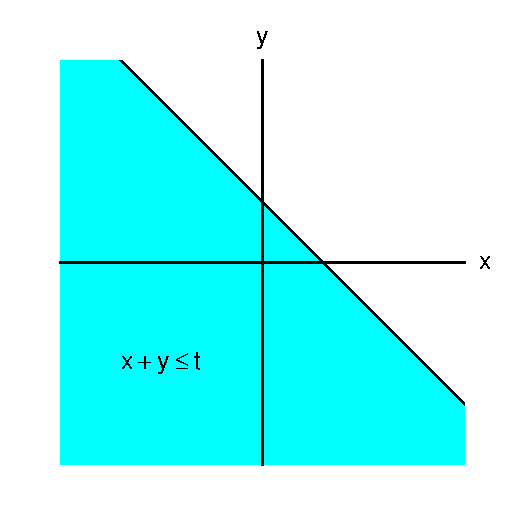
\includegraphics[scale=.5]{ch5_sumxy.pdf}
%\end{tabular}
%Therefore
%\begin{align*}
%f_{X+Y}(t) &= \frac{d}{dt} P(X+Y \leq t) 
%= \frac{d}{dt}\int_{-\infty}^\infty f_Y(y)F_X(t-y)\ dx\ dy \\
%&=\int_{-\infty}^\infty \frac{d}{dt}f_Y(y)F_X(t-y)\ dx\ dy 
%=\int_{-\infty}^\infty f_Y(y)f_X(t-y)\ dx\ dy
%\end{align*}
%\end{frame}

% Verify pdf of normal

% find gamma(1/2)

% calculate variance of hypergeometric

\begin{frame}{Convergence of Sample Means}
Suppose we generate a sequence of independent Bernoulli random variables $X_1, X_2, \dots$ with $p=.5$ and take the sample mean $\overline{X}=\frac1n\sum_{i=1}^n X_i$ using  larger and larger sample sizes.
\begin{center}
\vspace{0cm}
\begin{tabular}{p{3.5cm}p{7cm}}
\vspace{0cm}
\begin{tabular}{l|l}
$X_i$ & $\overline{X}$ \\ \hline
0 & 0 \\
1 & 1/2 \\
1 & 2/3 \\
0 & 2/4 \\
0 & 2/5 \\
0 & 2/6 \\
0 & 2/7 \\
1 & 3/8 \\
1 & 4/9 \\
0 & 4/10
\end{tabular}
&
\vspace{-.2cm}
{\animategraphics[width=6.5cm,height=6.5cm]{6}{ch4_lln_bern}{1}{100}}
\end{tabular}
\end{center}
\end{frame}

\begin{frame}{Convergence of Sample Means}
Let's try doing the same thing using standard uniform random variables.

\begin{center}
\vspace{0cm}
\begin{tabular}{p{3.5cm}p{7cm}}
\vspace{0cm}
\begin{tabular}{l|l}
$X_i$ & $\overline{X}$ \\ \hline
0.771 & 0.771 \\ 
0.409 & 0.590 \\ 
0.636 & 0.605 \\ 
0.291 & 0.527 \\ 
0.251 & 0.472 \\ 
0.099 & 0.409 \\ 
0.922 & 0.483 \\ 
0.990 & 0.546 \\ 
0.031 & 0.489 \\ 
0.113 & 0.451 \\ 
\end{tabular}
&
\vspace{-.2cm}
{\animategraphics[width=6.5cm,height=6.5cm]{6}{ch4_lln}{1}{100}}
\end{tabular}
\end{center}
\end{frame}


\begin{frame}{Convergence of Sample Means}
Let's try doing the same thing using exponential random variables with mean $\mu=10$:
\begin{center}
\vspace{0cm}
\begin{tabular}{p{3.5cm}p{7cm}}
\vspace{0cm}
\begin{tabular}{l|l}
$X_i$ & $\overline{X}$ \\ \hline
11.24 & 11.24 \\ 
3.73 & 7.49 \\ 
13.13 & 9.37 \\ 
0.97 & 7.27 \\ 
3.19 & 6.46 \\ 
4.05 & 6.05 \\ 
12.69 & 7.00 \\ 
4.11 & 6.64 \\ 
6.77 & 6.66 \\ 
7.45 & 6.73 \\ 
\end{tabular}
&
\vspace{-.2cm}
{\animategraphics[width=6.5cm,height=6.5cm]{6}{ch4_lln_exp}{1}{100}}
\end{tabular}
\end{center}
\end{frame}

\begin{frame}{Law of Large Numbers}
A result in probability theory guarantees that this works no matter what the distribution of the $X_i$ is, as long as $E(X_i)$ exists. For instance, the $X_i$ could be Bernoulli, geometric, normal, hypergeometric, binomial, or just about anything else we could imagine. 
\begin{block}{Law of Large Numbers}
Let $X_1,X_2,\dots$ be independent, identically distributed (iid) random variables with mean $\mu$. Then as $n\to\infty$, the sample mean $\overline{X}$ converges to $\mu$ with probability 1.
\end{block}
\end{frame}

\begin{frame}{Sample Mean of iid Random Variables}
Let $X_1,\dots, X_n$ be independent, identically distributed (iid) random variables with mean $\mu$ and variance $\sigma^2$. Let $\overline{X}$ be the sample mean 
$$\overline{X}=\frac1n\sum_{i=1}^n X_i = \frac1n(X_1+\cdots+X_n)$$

\pause\vspace{-.1cm} We can compute the expected value and variance of $\overline{X}$:
\begin{align*}
E(\overline{X}) &= E\left(\frac1n\sum_{i=1}^n X_i\right)
\uncover<3->{= \frac1n \sum_{i=1}^n E(X_i)}
\uncover<4->{= \frac1n \sum_{i=1}^n \mu }
\uncover<5->{= \frac1n(n\mu) }
\uncover<6->{= \mu\\[.1cm]}
\uncover<7->{V(\overline{X}) &= V\left(\frac1n\sum_{i=1}^n X_i\right) }
\uncover<8->{= \frac1{n^2} \sum_{i=1}^n V(X_i) }
\uncover<9->{= \frac1{n^2}\sum_{i=1}^n \sigma^2 }
\uncover<10->{= \frac1{n^2}(n\sigma^2) }
\uncover<11->{= \frac{\sigma^2}n}
\end{align*}
\uncover<12->{So the expected value of the sample mean $\overline{X}$ is $\mu$, the same as the expected value of each summand. However, the standard deviation $\sigma/\sqrt{n}$ of $\overline{X}$ decreases as we increase the sample size $n$.}
\end{frame}


\begin{frame}{Histogram of Sample Means}
\hspace*{-.3cm}\begin{tabular}{@{}p{5cm}p{7cm}}
\vspace{0cm}
Simulate a standard uniform random variable 20000 times and draw the histogram.

\vspace{.2cm}
\pause Now simulate standard uniform random variables $X_1$ and $X_2$ and compute the sample mean $\overline{X}=\frac12(X_1+X_2)$; do this 20000 times and draw the histogram.

\pause \vspace{.2cm}
Now repeat this using larger sample sizes: draw the histogram of 20000 simulations of $\overline{X}=\frac1n(X_1+\cdots+X_n)$, for $n=1,2,3,\dots,10$.

\pause\vspace{.2cm}
The histogram appears to approach a normal distribution.
 &
\vspace{0cm}
{\animategraphics[width=7cm,height=7cm,controls]{2}{ch4_clt_unif_hist}{1}{10}}
\end{tabular}
\end{frame}

\begin{frame}{Histogram of Sample Means}
Now repeat this but instead of simulating standard uniform random variables, use exponential random variables with $\mu=1$:

\begin{center}
\animategraphics[width=9cm,height=6cm,controls]{2}{ch4_clt_exp_hist}{1}{10}
\end{center}
\end{frame}

\begin{frame}{Central Limit Theorem}
A powerful result of probability theory guarantees that in general, if $n$ is large, then the sample mean $\overline{X}$ is approximately normal: 
%with mean $\mu$ and standard deviation $\sigma/\sqrt{n}$.
\begin{block}{}
Let $X_1,X_2,\dots$ be independent, identically distributed (iid) random variables with mean $\mu$ and standard deviation $\sigma$. Then
$$\lim_{n\to\infty} P\left(a \leq \frac{\overline{X}-\mu}{\sigma/\sqrt{n}} \leq b\right) = P(a \leq Z\leq b)=\Phi(b)-\Phi(a)$$
where $Z$ is a standard normal random variable.
\end{block}
\end{frame}

\begin{frame}{Distribution of Sample Means}
Compare the pdf of a the sample mean $\overline{X}$ of standard uniform random variables with the pdf of a normal random variable as specified in the Central Limit Theorem:
\animategraphics[width=10cm,height=6cm,controls]{2}{ch4_clt_unif}{1}{10}
\end{frame}

\begin{frame}{Distribution of Sample Means}
Compare the pdf of a the sample mean $\overline{X}$ of exponential random variables (with $\mu=10$) with the pdf of a normal random variable as specified in the Central Limit Theorem:
\animategraphics[width=10cm,height=6cm,controls]{2}{ch4_clt_exp}{1}{30}
\end{frame}

\begin{frame}{Sums of Random Variables}
Given iid random variables $X_1,\dots, X_n$  with mean $\mu$ and standard deviation $\sigma$, the Central Limit Theorem tells us that if $n$ is large, then the sample mean $\overline{X}=\frac1n(X_1+\cdots+X_n)$ is approximately normal.
% with mean $\mu$ and standard deviation $\sigma/\sqrt{n}$.

\vspace{.2cm}\pause
It follows that the sum $X_1+\cdots+X_n$ is also approximately normal, since the sum is the same as $\overline{X}$ scaled by a factor of $n$.
% but with mean $n\mu$ and standard deviation $n\cdot\sigma/\sqrt{n} = \sigma\sqrt{n}$.

\vspace{.2cm}\pause 
Examples:
\begin{itemize}
\pause\item A binomial is a sum of iid Bernoulli random variables.
\pause\item A negative binomial is a sum of iid geometric random variables.
\pause\item A Poisson$(\mu)$ random variable, where $\mu$ is an integer, is a sum of iid Poisson(1) random variables.
\end{itemize}
\pause So all of these examples may be approximated as normal if $n$ is large enough.
\end{frame}

\begin{frame}{Normal Approximation to Binomial}
Compare the pmf of a binomial random variable (with $p=.4$) to the pdf of the corresponding normal random variable:
\animategraphics[width=10cm,height=6cm,controls]{3}{ch4_clt_bern}{1}{27}
\end{frame}

\begin{frame}{Normal Approximation to Poisson}
Compare the pmf of a Poisson random variable to the pdf of the corresponding normal random variable:
\animategraphics[width=10cm,height=6cm,controls]{3}{ch4_clt_pois}{1}{18}
\end{frame}

\begin{frame}{Example}
\begin{block}{}
Bob is a candidate for political office in a large city and must take more than half the votes in order to win the election. Suppose a poll finds that 170 of 300 randomly sampled voters favor Bob. Approximate the probability that the poll would find so many voters favoring Bob if the true proportion were only .5.
\end{block}
\pause
Solution: The number $X$ of sampled voters favoring Bob is a hypergeometric random variable; but since the population is large, we may approximate $X$ as binomial, $\Bin(300,.5)$.

\vspace{.2cm}\pause
The Central Limit Theorem implies that $X$ is approximately normal, with mean
$\mu = np=150$ and standard deviation $\sigma=\sqrt{np(1-p)}=\sqrt{75}\approx 8.66$.
\pause
\begin{align*}
P(X \geq 170) &\approx P(8.66Z+150 \geq 170) \\
\uncover<5->{&\approx P(Z \geq 2.31) \\}
\uncover<6->{&= P(Z\leq -2.31)} 
\uncover<7->{ = \Phi(-2.31) }
\uncover<8->{\approx .0104}
\end{align*}
\end{frame}

\begin{frame}{Example}
\begin{block}{}
A Geiger counter placed next to a certain radioactive specimen clicks an average of 90 times per minute. Over a 10 minute period, approximate the probability that it would click 800 times or less.
\end{block}
\pause Solution: The number of clicks $X$ in a 10 minute period has a Poisson distribution with mean $\mu=900$. The variance of $X$ is $V(X)=\mu=900$, so the standard deviation is $\sigma=\sqrt{900}=30$.

\pause 
\vspace{.2cm}
Since $\mu$ is large, the distribution of $X$ is approximately normal. So we can approximate $X$ as $30Z+900$ where $Z$ is a standard normal random variable. \pause Then
\begin{align*}
P(X \leq 800) &\approx P(30Z+900 \leq 800) \\
\uncover<4->{&\approx P(Z \leq -3.33)}
\uncover<5->{ = \Phi(-3.33) }
\uncover<6->{\approx .0004 }
\end{align*}
\end{frame}

\begin{frame}{Summary}
\begin{itemize}
\item \textbf{Joint pmf} of discrete random variables $X$ and $Y$: $$f(x,y)=P(X=x \cap Y=y)$$
\item \textbf{Joint pdf} of continuous random variables $X$ and $Y$: 
$$P(a \leq X \leq b \cap c \leq Y \leq d)=\int_{a}^b\int_{c}^d f(x,y)\ dy\ dx$$
\item \textbf{Covariance} of two random variables $X$ and $Y$:
\begin{itemize}
\item Definition: $\Cov(X,Y) = E[(X-\mu_X)(Y-\mu_Y)]$
\vspace{.08in}
\item Shortcut formula: $\Cov(X,Y)=E(XY)-E(X)E(Y)$
\item Properties:
%\begin{block}{}
\begin{enumerate}
\item $\Cov(X,X) = V(X)$
\item $\Cov(Y,X) = \Cov(X,Y)$
\item $\Cov(cX,Y) = c\Cov(X,Y)$
\item $\Cov(X+Y,Z) = \Cov(X,Z)+\Cov(Y,Z)$
\end{enumerate}
%\end{block}
\end{itemize}
\end{itemize}
\end{frame}

\begin{frame}{Summary}

\begin{itemize}
\item \textbf{Correlation}: $$\Corr(X,Y)=\frac{\Cov(X,Y)}{\sigma_X\sigma_Y}$$
\item \textbf{Sample Mean}: $$\overline X = \frac1n\sum_{i=1}^n X_i$$
\begin{itemize}
\item If $E(X_i)=\mu$ and $V(X_i)=\sigma^2$, then 
\begin{align*}
E(\overline X)&=\mu\\
V(\overline X)&=\frac{\sigma^2}n
\end{align*}
\end{itemize}
\item \textbf{Law of Large Numbers}: As the sample size $n$ increases, $\overline{X}$ converges to $E(X)$.
\item \textbf{Central Limit Theorem}: As the sample size $n$ increases, $\overline X$ becomes approximately normal. More precisely, $\frac{\overline{X}-E(X)}{\sigma/\sqrt{n}}$ converges to a standard normal distribution.
\end{itemize}
\end{frame}

\end{document}